\documentclass[times, utf8, zavrsni]{fer}
\usepackage{booktabs}
\usepackage{graphicx}
\usepackage[]{algorithm2e}
\usepackage{caption}
\usepackage{multirow}
\graphicspath{{/home/mateo/Git/Kraken_memory_improvement/Pictures/}}
\begin{document}

% TODO: Navedite broj rada.
\thesisnumber{5133}

% TODO: Navedite naslov rada.
\title{Algoritam staničenja velike baze podataka genoma}

% TODO: Navedite vaše ime i prezime.
\author{Mateo Stjepanović}

\maketitle

% Ispis stranice s napomenom o umetanju izvornika rada. Uklonite naredbu \izvornik ako želite izbaciti tu stranicu.
\izvornik

% Dodavanje zahvale ili prazne stranice. Ako ne želite dodati zahvalu, naredbu ostavite radi prazne stranice.
\zahvala{Zahvaljujem mentorici doc.\ dr.\ sc.\ Mirjana Domazet-Lošo na podršci.}

\tableofcontents

\chapter{Uvod}
Bioinformatika je interdisciplinarna znanost koja se bavi razvojem programa i metoda za interpretiranje bioloških podataka. Spaja matematiku, statistiku, računalnu znanost te druge prirodno matematičke znanosti. U posljednjem desetljeću bioinformatika kao znanost doživaljava veliki porast, te kao takva uspjeva mapirati genome mnogih živih bića.\\
U navedenom porastu najviše se ističu metode analiziranja genoma, te, spajanjem statističkih analiza i algoritama iz područja računalne znanosti, metode određivanja položaja istih u taksonomskom stablu. Upravo u tom području postoje mnogi alati koji su razvijeni upravo s ciljem poboljšanja točnosti određivanja taksonomskog stabla novoj, nepoznatoj, jedinki.\\ Za većinu jedinki u uzorku su vrsta, rod i više razine stabla nepoznati. Ako je jedinka potpuno nepoznata tada će se klasificirati kao nova nepoznata vrsta te se neće dalje klasificirati. U velikom broju slučajeva će postojati neke sličnosti sa nekim već određenim vrstama, te je potrebno pronaći te sličnosti kako bi se sjedinka uspješno klasificirala. Za to služe razni algoritmi poravnanja. Jedan od tih je BLAST. Postoje druge metode i programi koji pospješuju učinkovitost BLAST-a uvođenjem metoda strojnog učenja. Iako bolje preciznosti ti programi imaju jednu veliku manu. Vrijeme potrebno za klasificiranje podatka je jako veliko, stoga su više manje neiskoristivi. \\Tu na scenu nastupa alat za klasifikaciju metagenoma nazvan Kraken(Derrick E. Wood i Steven L.).
\\{\textit{Kraken is ultrafast and high accurate program for assigning taxonomic labels to metagenomic DNA sequences.}\footnote[1]{Wood and Salzberg: \textbf{Kraken: ultrafast metagenomic sequence classification using exact alignments.} \textit{Genome Biology} 2914 15:R46}
\\Za razliku od alata koji su pokušali poboljšati preciznost BLAST algoritma, te time izgubili na brzini, Kraken je jedan od rijetkih alata koji postiže točnost koja premašuje onu u BLAST algoritmu, s time da ne gubi na brzini izvođenja. Rad Krakena se sastoji od toga da se ulazni podatak "razbija" na k-mere, te se minimizer algoritmom traže oni k-meri koji imaju istu vrijednost minimzer-a. Tada se taj podatak uspoređuje s podacima u Kraken-ovoj bazi podataka, s tim da je baza sortirana na način da su podaci sa istim minimizerom smješteni jedan pored drugog, tako da se pretraživanje jako pospješuje i ubrzava. Autori alata su shvatili da Kraken može naići an problem prilikom izvođenja na računalu s ograničenim resursima, točnije na računalu s RAM-om ispod 70GB. Iz tog razloga je razvijena MiniKraken baza podataka koja je sa prvotnih 70GB podataka smanjena na 4GB.
\begin{table}[htb]
	\centering
	\resizebox{\textwidth}{!}{%
		\begin{tabular}{|llcccccc|}
			\hline
			\multicolumn{1}{|c}{} & \multicolumn{1}{c}{}  & \multicolumn{2}{c}{HiSeq}                                       & \multicolumn{2}{c}{MiSeq}                                       & \multicolumn{2}{c|}{simBA-5}                                     \\
			\multicolumn{2}{|l}{Classifier}              & \multicolumn{1}{l}{Precision} & \multicolumn{1}{l}{Sensitivity} & \multicolumn{1}{l}{Precision} & \multicolumn{1}{l}{Sensitivity} & \multicolumn{1}{l}{Precision} & \multicolumn{1}{l|}{Sensitivity} \\ \hline
			Megablast             & \multicolumn{1}{l|}{} & \multicolumn{1}{c|}{99.03}    & \multicolumn{1}{c|}{79.00}      & \multicolumn{1}{c|}{92.44}    & \multicolumn{1}{c|}{75.76}      & \multicolumn{1}{c|}{96.93}    & 93.67                            \\ \hline
			NBC                   & \multicolumn{1}{l|}{} & \multicolumn{1}{c|}{82.33}    & \multicolumn{1}{c|}{82.33}      & \multicolumn{1}{c|}{77.78}    & \multicolumn{1}{c|}{77.78}      & \multicolumn{1}{c|}{97.64}    & 97.64                            \\ \hline
			PhymmBL               & \multicolumn{1}{l|}{} & \multicolumn{1}{c|}{79.14}    & \multicolumn{1}{c|}{79.14}      & \multicolumn{1}{c|}{76.21}    & \multicolumn{1}{c|}{76.21}      & \multicolumn{1}{c|}{96.11}    & 96.11                            \\ \hline
			PhymmBL65             & \multicolumn{1}{l|}{} & \multicolumn{1}{c|}{99.13}    & \multicolumn{1}{c|}{73.95}      & \multicolumn{1}{c|}{92.47}    & \multicolumn{1}{c|}{73.03}      & \multicolumn{1}{c|}{99.08}    & 95.45                            \\ \hline
			Kraken                & \multicolumn{1}{l|}{} & \multicolumn{1}{c|}{99.20}    & \multicolumn{1}{c|}{77.15}      & \multicolumn{1}{c|}{94.71}    & \multicolumn{1}{c|}{73.46}      & \multicolumn{1}{c|}{99.90}    & 91.25                            \\ \hline
			Kraken-Q              & \multicolumn{1}{l|}{} & \multicolumn{1}{c|}{99.12}    & \multicolumn{1}{c|}{76.31}      & \multicolumn{1}{c|}{94.69}    & \multicolumn{1}{c|}{70.41}      & \multicolumn{1}{c|}{99.92}    & 89.54                            \\ \hline
			MiniKraken            & \multicolumn{1}{l|}{} & \multicolumn{1}{c|}{99.44}    & \multicolumn{1}{c|}{66.12}      & \multicolumn{1}{c|}{97.41}    & \multicolumn{1}{c|}{67.95}      & \multicolumn{1}{c|}{99.95}    & 65.87                            \\ \hline
			MiniKraken-Q          & \multicolumn{1}{l|}{} & \multicolumn{1}{c|}{99.36}    & \multicolumn{1}{c|}{65.67}      & \multicolumn{1}{c|}{97.32}    & \multicolumn{1}{c|}{65.84}      & \multicolumn{1}{c|}{99.98}    & 65.31                            \\ \hline
			Kraken-GB             & \multicolumn{1}{l|}{} & \multicolumn{1}{c|}{99.51}    & \multicolumn{1}{c|}{93.75}      & \multicolumn{1}{c|}{98.48}    & \multicolumn{1}{c|}{86.23}      & \multicolumn{1}{c|}{99.48}    & 91.13                            \\ \hline
		\end{tabular}%
	}
	\caption{Klasifikacija roda za tri metagenoma}
	\label{StatRez}
\end{table}


\chapter{Definiranje problema}
Uz već spomenutost rješenja problema korištenja velike količine resursa, nailazi se na problem koji će se pokušati riješiti tijekom ovog rada.
% Please add the following required packages to your document preamble:
% \usepackage{graphicx}
\begin{table}[hbp]
	\centering
	\resizebox{\textwidth}{!}{%
		\begin{tabular}{|llcccccc|}
			\hline
			\multicolumn{1}{|c}{} & \multicolumn{1}{c}{} & \multicolumn{2}{c}{HiSeq} & \multicolumn{2}{c}{MiSeq} & \multicolumn{2}{c|}{simBA-5} \\
			\multicolumn{2}{|l}{Classifier} & \multicolumn{1}{l}{Precision} & \multicolumn{1}{l}{Sensitivity} & \multicolumn{1}{l}{Precision} & \multicolumn{1}{l}{Sensitivity} & \multicolumn{1}{l}{Precision} & \multicolumn{1}{l|}{Sensitivity} \\ \hline
			Kraken & \multicolumn{1}{l|}{} & \multicolumn{1}{c|}{99.20} & \multicolumn{1}{c|}{77.15} & \multicolumn{1}{c|}{94.71} & \multicolumn{1}{c|}{73.46} & \multicolumn{1}{c|}{99.90} & 91.25 \\ \hline
			MiniKraken & \multicolumn{1}{l|}{} & \multicolumn{1}{c|}{99.44} & \multicolumn{1}{c|}{66.12} & \multicolumn{1}{c|}{97.41} & \multicolumn{1}{c|}{67.95} & \multicolumn{1}{c|}{99.95} & 65.87 \\ \hline
		\end{tabular}%
	}
	\caption{Isječak iz Tablice 1.1}
	\label{IsjecakTablice}
\end{table}

Iako se iz dane tablice vidi da se preciznost korištenjem MiniKraken baze podataka neznatno povećala u odnosu na Kraken bazu podataka. S druge strane osjetljivost jako opada. Osjetljivost predstavlja mjeru koja određuje postotak uočenih lažno negativnig podataka, tj. predstavlja postotak točno kvalificiranih podataka koji su uistinu tako i predstavljeni. S druge strane precizonst predstavlja izbjegavanje lažno pozitivnih podataka, tj. koliko podataka je uočeno da ne pripadaju nekoj skupini, s tim da oni uistinu ne pripadaju toj skupini.\\Ideja ovog rada je da se algoritmima sličnim algoritmima straničenja osposobi računalo s ograničenim resursima za rad s bazom podataka čija veličina uvelike nadilazi količinu RAM-a raspoloživog na računalu. Prvotno je potrebno podjeliti bazu podataka na više manjih koje će se moći uspješno učitati u memoriju te pretražiti. Ideja je iskoristiti "kontejnere" k-mera koji su određeni svaki jedinstvenom minimizer vrijednosti, te pomoću binarnog pretraživanja indeksa učitavati samo onu bazu podataka pomoću koje je moguće klasificirati podatak u taksonomsko stablo. Želeći se približit straničenju, predstavit će se samo iteriranje po indeksima te učitavati slijedno baze podataka i pretraživati svaku.
\chapter{Strukture podataka i algoritmi u Kraken-u}
\subsection{Baza podataka}
\subsubsection{Kreiranje baze podataka}

Nastanak baze podataka se događa u nekoliko koraka. Za početak se sa NCBI-a preuzimaju biblioteke koje sadrže trenutno poznate vrste. Budući da pretraživanje baze podataka u Kraken-u osniva na k-merima potrebno je proizvesti k-mere za svaki podataka u bazi podataka. Za to služi alat naziva Jellyfish(Guillaume Marçais i Carl Kingsford) koji računa k-mere zadane duljine 31 ( korisnik također može zadati duljinu k-mera).\\Jellyfish je alat za brzo i memorijski povoljno prebrojavanje podnizova u danom nizu. Za potrebe prilagodbe svim resursima za Jellyfish postoje opcije za brzo izračunavanje koje je memorijski zahtjevnije, te ono sporije ali memorijski ne toliko zahtjevno. U kontekstu bioinformatike Jellyfish se koristi za prebrojavanje k-mera u zadanom metagenomu. Sam rad se bazira na hash tablici koja je osposobljena za paralelan rad preko više CPU-a. Hash tablica se sastoji od para (ključ,vrijednost), gdje je ključ zadani k-mer a vrijednost je broj njegovog ponavljanja u metagenomu.
	 	
\begin{table}[hbp]
	\centering
	\caption{Prikaz niza te njegovih k-mera (k = 4)}
	\label{Prikaz k-mera}
	\begin{tabular}{llllllllll}
		Ulaz:  &           & \multicolumn{8}{l}{AGATCGAGTG}                            \\
		4-mer: & \multicolumn{2}{l}{} & AGAT & GATC & ATCG & TCGA & CGAG & GAGT & AGTG
	\end{tabular}
\end{table}
Nakon rada Jellyfish-a u bazu se spremaju 4 bajtne vrijednosti k-mera te se kreira identifikacijska oznaka za svaki podataka. Tada program kreiranja baze podataka ponovno prolazi kroz istu, te za svaki identifikator podatka izračunava njegov LCA(\textit{Najmanji zajednički predal}), te ga sprema u bazu podataka zajedno s identifikatorom i njegovim k-merima.
\subsubsection{Strukture baze podataka}
Gore navedeni proces klasificiranja ulaznog genoma pomoću baze podataka se , već navedeno, bazira na pretraživanju k-mera. Baza podataka se sastaoji od identifikacijskih oznaka svakog podatka u njoj, njihovog izračunatog najmanjeg zajedničkog pretka, te k-mera koje on tvori.\\
\begin{figure}[hbp]
	\centering
	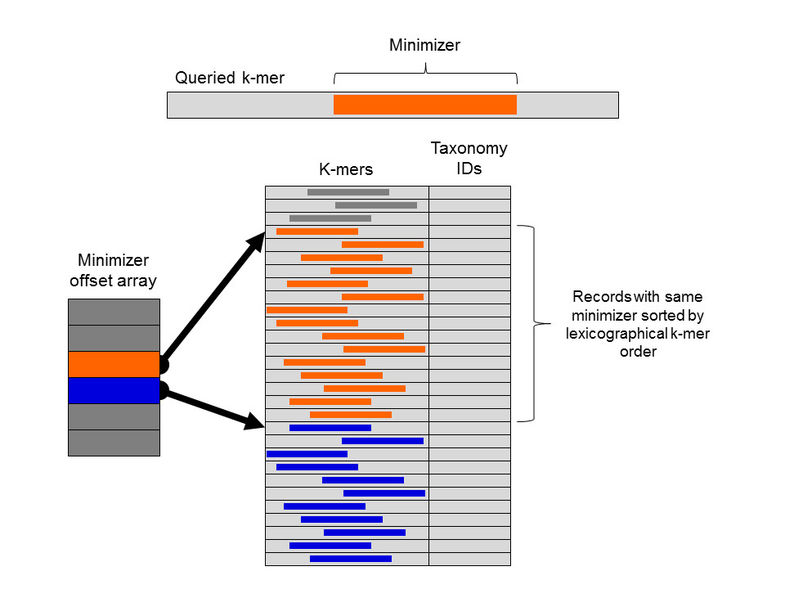
\includegraphics[width=\textwidth]{DbStructure.jpg}
	\caption{Prikaze strukture baze podataka}
	\label{BazaPodataka}
\end{figure}

S ciljem poboljšanja brzine pretraživanja, uvodi se algoritam indeksiranja i raspoređivanja poznat pod imenom Minimizer (Roberts M, Hayes W, Hunt B, Mount s, te Yorke J.).
 

\begin{algorithm}[H]
	\SetAlgorithmName{Algoritam}{algoritam}{List of algoritam}
	ptr <- pokazivač\_na\_k-mer\;
	k\_ct <- brojač kontejnera\;
	vrijednosti <- 1ull << (nt * 2)\;
	\While{brojač je različit od broja kontejnera}{
		brojač++\;
		dohvati\_k-mer(ptr)\;
		ključ <- izračunaj\_ključ()\;
		b\_brojac[ključ]++\;		
	}
	b\_ofset\_ofset[vrijednosti +1]\;
	\For{i < vrijednosti}{
		b\_ofset = b\_ofset[i-1]+b\_brojac[i-1]\;
	}
	indeks(b\_ofset)\;
	\caption{Računanje indeksa kontejnera}
\end{algorithm}

Prilikom sortiranja i indeksiranja se stvaraju svojevrsni kontejneri koji sadržavaju one podatke čiji k-meri imaju iste minimizer vrijednosti.Tom idejom se poboljšava pretraživanje na način da se za svaki ulazni podataka računaju njegovi k-meri te njegove minimizer vrijednosti, te se pretragom liste indeksa dohvaća samo onaj kontejner koji sadrži istu minimizer vrijednost.


\newpage
\subsection{Algoritam klasifikacije podataka}

Klasificiranje ulaznog podatka se odvija na više razina. Za početak se za ulazni genom računaju svi njegovi k-meri ( koje korisnik može postaviti, ili biti zadani). K-mere ulaznog skupa ćemo na dalje označavati sa K(S). Zatim se za svaki k-mer kreiraju njegove LCA vrijednosti, tj. traži se onaj podatak u taksonomskom stablu, koji predstavlja prvog pretka tog k-mera. Od svih k-mera se tada kreira stablo koje predstavlja sve moguće klasifikacije za dani genom, a koje su dobivene upravo navedenim algoritmom. Svaka vrijednost u stablu ima izračunatu vrijednost koja predstavlja koliko k-mera se podudara sa tim podatkom. Ako za neki k-mer ne postoji poznati LCA , tada se on neće ni stavljati u navedeno stablo. Način rada koji uvodi tečine za svaki čvor u stablu omogućuje veliku točnost u radu Krakena-a, tako da ako postoji neki put u stablu koji je pogrešan a težine su jako male, on će se zanemariti. Ako postoje dva puta u stablu koja imaju iste težine tada se samo za te podatke ponovno računa LCA te se pokušava odrediti koji put zapravo predstavlja točnu klasifikaciju.

\begin{figure}[!htbp]
	\centering
	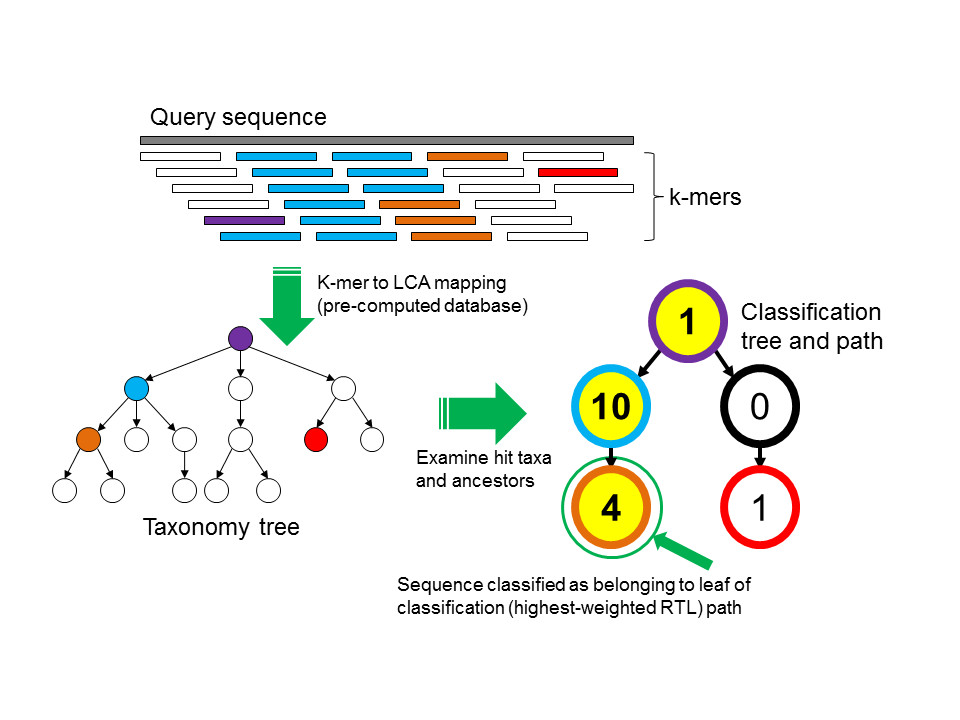
\includegraphics[width=\textwidth]{Work.jpg}
	\caption{Prikaza klasifikacije podataka}
	\label{Klasifikacija}
\end{figure}

Iz slike 3.2 se može vidjeti način rada algoritma. Nakon određivanja k-mera u prvom dijelu slike se pokušavaju one klasificirata na LCA pomoću već izvedene baze podataka. Nakon toga se računaju težine te taj dio je predstavljen u desnom prikazu na slici. Iako postoje dva puta do lista. prihvaća se samo ovaj lijevi jer on ima veće težine, tj. broj k-mera koji se podudaraju s ovim putom je mnogo veći nego na desnom putu.


\subsection{LCA(\textit{Lower Common Ancestor})}
LCA(\textit{Lower common ancestor}) je jedan od osnovnih algoritamskih problema u strukturama stabala.A označava pronalazak čvora u stablu koji je najudaljeniji od korijena stabla, te je zajednički čvorovima \textit{u} i \textit{v}. Prvu ideju i definiciju LCA dali su Alfred Aho, John Hopcroft i Jeffrey Ullman 1973. godine u svom radu \textit{On finding lowest common ancestors in trees}. Zbog svoje složenosti te raznolike primjenjivosti ovaj problem je još uvijek aktualan, te se i danas objavljuje mnogo članaka i radova na tu temu.
\begin{figure}[!htbp]
	\centering
	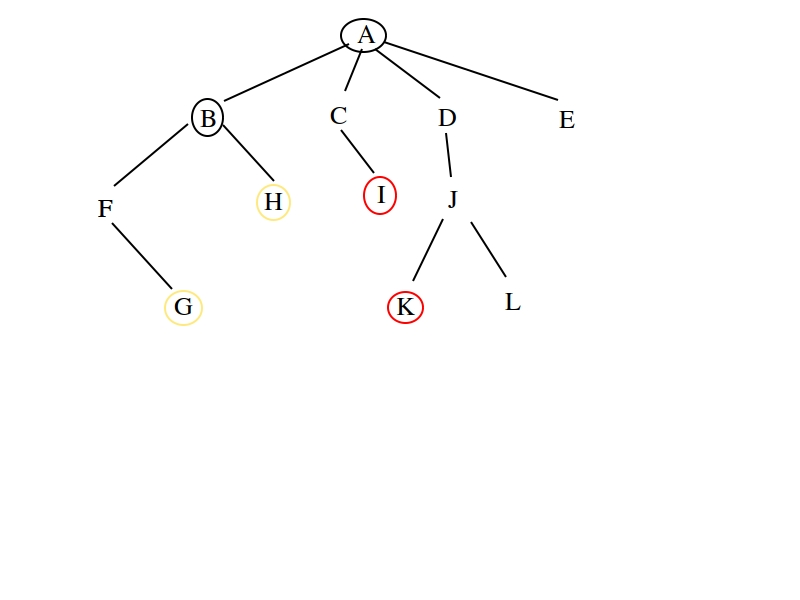
\includegraphics[width=\textwidth]{lca.jpg}
	\caption{Prikaz stabla i LCA vrijednosti}
	\label{LCA}
\end{figure}

Na slici 3.3 se nalazi prikaz strukture stabla te su bojama označeni listovi za koje želimo naći najmanjeg zajedničkog pretka (LCA). Crno obojani čvorovi su čvorovi koji su LCA tim dvama listovima. Tako je za listove H i G najmanji zajednički predak čvor B, dok je za listove I i K najmanji zajednički predak A. U radu \textit{On finding lowest common ancestors in trees} 1973. godine je predstavljen sljedeći pseudokod za određivanje najmanjeg zajedničkog pretka.
\newline
\newline
\begin{algorithm}[H]
	
	\SetAlgorithmName{Algoritam}{algoritam}{List of algoritam}
	
	procedure getancestor(u,i)\footnote[1]{A.V.Aho, J.E.Hopcroft, J.D.Ullman, \textbf{On finding lowest common ancestor in trees} \textit{ACM New York, NY, USA ©1973}}:\\

	
		\If{ancestor(u,i-1) = undefined then;}{
			ancestor(u,i) <- getancestor(getancestor(u,i-1),i-1)\;
		}
		resultis ancestor(u,i)\;
	\caption{Dohvaćanje pretka}
	\label{LCA algoritam 1}
\end{algorithm}
Algoritam 2 predstavlja metodu getancestor(u,i), koja prima čvor \textit{u} te dubinu \textit{i}. Funkcija dohvaća 2\^ i-tog pretka te ga stavlja u niz. \textit{Getancestor} se poziva tijekom traženja najmanjeg zajedničkog pretka
\newline
\newline
\begin{algorithm}[H]

	\SetAlgorithmName{Algoritam}{algoritam}{List of algoritam}
		procedure find(u,v,i,d)\footnote[2]{A.V.Aho, J.E.Hopcroft, J.D.Ullman, \textbf{On finding lowest common ancestor in trees} \textit{ACM New York, NY, USA ©1973}}:\\
		\eIf{i = 0}{
			resultis ancestor(u,0)\;
		}{
			\eIf{getancestor(u,i-1)=getancestor(v,i-1)}{
				resultis find(u,v,i-1,d)\;
			}{
				resultis find(getancestor(u,i-1),getancestor(v,i-1),min(i-1,|\_log(d-2\^(i-1))\_|),d-2\^(i-1))\;
			}
		}
	\caption{Pronalazak LCA}
	\label{LCA algorithm 2}
	
\end{algorithm}

Algoritam 3 predstavlja metodu koja pronalazi najmanjeg zajedničkog pretka za ulazne podatke \textit{u} i \textit{v} koji su na dubini \textit{d}. Početne pretpostavke su da je \textit{d} > 2 \^(i-1) te su im 2\^i-ti preci jednaki ili ne postoje.

\chapter{Algoritmi indeksiranja i pretrage}
\subsection{Minimizer - algoritam za reduciranje podataka}
Usporedba podataka je osnova moderne bioinformatike. Ona se danas temelji na metodi \textit{seed-and-extend}. Za svaki ulazni podatak se uzima samo jedan uzorak, te se on uspoređuje u bazi podataka. Ako se nađe poklapanje tada se taj uzorak proširuje na cijeli podatak te se ponovno uspoređuje. Da bi sve to funkcioniralo potrebno je uzeti uzorak za svaki podskup u jednom genomu, što , za kompleksnije genome, zauzima jako puno memorije.Na ideju rješenja su došli Michael Roberts, Wayne Hayes, Brian R. Hunt, Stephen M. Mount i James A. York u svom radu \textit{Reducing storage requirements for biological sequence comparison}. Koristi se isti način rada, tj.\textit{seed-and-extend}, uz razliku da se ne uzimaju svi uzorci, nego samo mali podskup jedinstvenih, nazvanih "minimizer-i".
\\ Navedeni algoritam sažimanja se koristi i u Kraken bazi podataka, te ju uvelike smanjuje i pospješuje brzinu izvođenja. Prilikom kreiranja MiniKraken baze podataka se koristi isti način rada, uz razliku da se odbacuje samo određeni postotak prvih i zadnjih vrijednosti. Da bi kontejneri u kojima su sadržani podaci s istim minimizer vrijednostima zadržao svojstvo kolekcije, potrebno je da su ti isti podaci normalno distribuirani, što se postiže brisanjem pola bitova prilikom ispitivanja jednakosti. S ciljem pospješenja brzine izvođenja, jer svako računanje minimizer vrijednosti je relativno skupo, prilikom klasifikacije podatka koristi se onaj kontejner koji je korišten prije, te ako k-meri nisu nađeni u njemu, računa se minimizer vrijednost. Ako je minimizer vrijednost jednaka kao u kontjerneru zaključuje se da se podatak ne može klasificirati, inače se pozicionira u dani kontejner te se ponovno vrši pretraga.

Postije dvije vrste minimizer-vrijednosti: unutarnje i vanjske. Svakoj od njih je srž računanja isti, tj. za ulazni niz se računaju svi njegovi k-meri za zadani k, te se iz njih tada bira onaj k-mer koji je leksikografski najmanji. 

\begin{figure}[htbp]
	\centering
	
	\begin{tabular}{l|l|llllllll|}
		\multicolumn{2}{l|}{Pozicija:}                                                                                       &  & 1 & 2 & 3 & 4          & 5          & 6          & 7 \\ \hline
		\multicolumn{2}{l|}{Ulazni niz:}                                                                                     &  & 2 & 3 & 1 & 0          & 3          & 4          & 3 \\ \hline
		\multicolumn{2}{l|}{\multirow{5}{*}{\begin{tabular}[c]{@{}l@{}}k-meri\\ s\\ podebljanim\\ minimizerom\end{tabular}}} &  & 2 & 3 & 1 &            &            &            &   \\
		\multicolumn{2}{l|}{}                                                                                                &  &   & 3 & 1 & 0          &            &            &   \\
		\multicolumn{2}{l|}{}                                                                                                &  &   &   & 1 & 0          & 3          &            &   \\
		\multicolumn{2}{l|}{}                                                                                                &  &   &   &   & \textbf{0} & \textbf{3} & \textbf{4} &   \\
		\multicolumn{2}{l|}{}                                                                                                &  &   &   &   &            & 3          & 4          & 3 \\ \hline
	\end{tabular}
	\caption{K-meri ulaznog niza s minimizer-om}
	\label{Minimizer}
\end{figure}

Slika 4.1 prikazuje način odabira minimizera za ulazni niz. Ulazni niz je podjeljen na 3-mere , a za računanje minimizer-a se koristi prozor od 5 k-mera. Korištenje prozora znači da se samo u 5 k-mera odjednom traži minimizer vrijednost. Budući da je \textit{034} leksikografksi najmanji podniz on se uzima kao zadani minimizer. Algoritam minimizer nam garantira da će dva niza koja su ista sadržavati barem jednu istu minimizer vrijednost.
\subsection{Binarno pretraživanje}
Za pretraživanje svakog kontejnera se koristi binarno pretraživanje. Binarno pretraživanje je jedan od osnovnih algoritama u računalnoj znanosti. Glavni zadatak algoritma je pronalazak vrijednosti u sortiranom nizu. Osnovna i glavna pretpostavka jest da je niz sortiran, u suprotnom sam algoritam nema smisla.
\newline
\newline
\begin{algorithm}[H]
	\SetAlgorithmName{Algoritam}{algoritam}{List of algoritam}
	binarno\_pretraživanje(niz,cilj):\\
	lo = 1, hi = size(niz)\;
	\While{lo <= hi}{
		mid = lo + (hi - lo) / 2\;
		\eIf{niz[mid] == cilj}{
			return mid\;
		}{
			\eIf{niz[mid] < cilj}{
				lo = mid + 1\;	
			}{
				hi = mid + 1\;
			}
		}
	}
	\caption{Binarno pretraživanje}
	\label{BinarnoP}
\end{algorithm}

Inicijalno je radni prostor binarnog pretraživanja cijeli ulazni niz. Tada se pozicionira na sredinu tog niza, te se ispituje je li vrijednost na sredini jednaka onoj koju mi tražimo. Ako je rezultat potvrdan izlazimo iz petlje te vraćamo poziciju te vrijednosti. U protivnom se ispituje odnos tražene vrijednosti i one koja je na sredini. Ako je vrijednost na sredini manja od tražene radni prostor postavljamo na onu polovicu koja se nalazi desno od indeksa, tj. prelazimo u  polovicu koja sadrži veće vrijednosti, u suprotnom se pozicioniramo na manju polovicu. Složenost binarnog pretraživanja je O(logN). Logaritam je sporo rastuća funkcija, stoga je binarno pretraživanje jako efikasan algoritam. Kao primjer za pretragu imenika od milion imena, pomoću binarnog pretraživanja bismo pronašli traženu vrijednost u najviše 21 korak.


\chapter{Pseudokod i razrada algoritma}


\chapter{Analiza učinkovitosti rješenja}
\chapter{Zaključak}
Zaključak.

\bibliography{literatura}
\bibliographystyle{fer}

\begin{sazetak}
Sažetak na hrvatskom jeziku.

\kljucnerijeci{Ključne riječi, odvojene zarezima.}
\end{sazetak}

% TODO: Navedite naslov na engleskom jeziku.
\engtitle{Title}
\begin{abstract}
Abstract.

\keywords{Keywords.}
\end{abstract}

\end{document}
